\documentclass[preprint,12pt]{elsarticle}
\usepackage[utf8]{inputenc}
\usepackage[T1]{fontenc}
\usepackage{lmodern}
\usepackage{amsmath,amssymb}
\usepackage{graphicx}
\usepackage{booktabs}
\usepackage{multirow}
\usepackage{enumitem}
\usepackage{xcolor}
\usepackage{tikz}
\usetikzlibrary{calc,positioning,arrows.meta}
\usepackage[most]{tcolorbox}
\usepackage{listings}
\usepackage{url}
\usepackage[hidelinks]{hyperref}
\usepackage{lineno}
\graphicspath{{figures/}}
\newcommand{\npapers}{3,274}
\newcommand{\npapersIncluded}{3,117}
\newcommand{\npapersThreeDCP}{1,176}
\newcommand{\nmixes}{29,626}
\newcommand{\nmeasurements}{236,199}
\newcommand{\nmeasurementsValued}{81,030}
\newcommand{\ncurves}{25,721}
\newcommand{\ncurvePoints}{155,211}
\newcommand{\nprintRuns}{7,420}
\newcommand{\nprintPapers}{928}
\newcommand{\nprintPrintable}{5,586}
\newcommand{\nprintNon}{902}
\newcommand{\nprintBorder}{932}
\newcommand{\nprintCollapses}{941}
\newcommand{\nprintSTF}{841}
\newcommand{\nprotocolRows}{1,507}
\newcommand{\nnMixesNorm}{28,001}
\newcommand{\nnFeatures}{138}
\newcommand{\nnModels}{36}
\newcommand{\nnTargets}{19}
\newcommand{\nrFailN}{146}
\newcommand{\nrFailPapers}{37}
\newcommand{\nrFailMedian}{1.39}
\newcommand{\nrFailPtf}{0.64}
\newcommand{\nrFailPsf}{2.87}
\newcommand{\nnTools}{16}
\newcommand{\nbenchCxN}{33}
\newcommand{\nbenchCxPassn}{33}
\newcommand{\nbenchCxPassrate}{1.000}
\newcommand{\nbenchCxToolok}{33}
\newcommand{\nbenchCxParamok}{33}
\newcommand{\nbenchCxNchecks}{105}
\newcommand{\nbenchCxFidelity}{0.996}
\newcommand{\nbenchCxNnumbers}{497}
\newcommand{\nbenchCxNuntraced}{6}
\newcommand{\nbenchCxCallsmedian}{3}
\newcommand{\nbenchCxToolerrors}{6}
\newcommand{\nbenchCxWallmedian}{39}
\newcommand{\nbenchCxWallpninety}{89}
\newcommand{\nbenchCxWallmax}{172}
\newcommand{\nbenchCxCost}{0}
\newcommand{\nbenchCxModel}{gpt-6-astra}
\newcommand{\nbenchCxIntokens}{6,203,134}
\newcommand{\nbenchCxOuttokens}{32,650}
\newcommand{\nbenchCxCachetokens}{5,389,952}
\newcommand{\nbenchCxControl}{0.378}
\newcommand{\nbenchCxTruthn}{6}
\newcommand{\nbenchCxTruthok}{6}
\newcommand{\nbenchCxFatal}{0}
\newcommand{\nbenchCsN}{33}
\newcommand{\nbenchCsPassn}{33}
\newcommand{\nbenchCsPassrate}{1.000}
\newcommand{\nbenchCsToolok}{33}
\newcommand{\nbenchCsParamok}{33}
\newcommand{\nbenchCsNchecks}{105}
\newcommand{\nbenchCsFidelity}{0.998}
\newcommand{\nbenchCsNnumbers}{596}
\newcommand{\nbenchCsNuntraced}{4}
\newcommand{\nbenchCsCallsmedian}{4}
\newcommand{\nbenchCsToolerrors}{6}
\newcommand{\nbenchCsWallmedian}{48}
\newcommand{\nbenchCsWallpninety}{111}
\newcommand{\nbenchCsWallmax}{142}
\newcommand{\nbenchCsCost}{0}
\newcommand{\nbenchCsModel}{gpt-6-sol}
\newcommand{\nbenchCsIntokens}{7,150,793}
\newcommand{\nbenchCsOuttokens}{55,050}
\newcommand{\nbenchCsCachetokens}{6,284,288}
\newcommand{\nbenchCsControl}{0.445}
\newcommand{\nbenchCsTruthn}{6}
\newcommand{\nbenchCsTruthok}{6}
\newcommand{\nbenchCsFatal}{0}
\providecommand{\nbenchCxModel}{(pending)}

% ---------------------------------------------------------------- transcript boxes
\definecolor{userbg}{HTML}{FFF4D6}
\definecolor{agentbg}{HTML}{F3F4F6}
\definecolor{toolbg}{HTML}{E8F1FB}
\newtcolorbox{userbox}{enhanced, colback=userbg, colframe=userbg!60!black, boxrule=0.4pt, arc=2pt, left=5pt, right=5pt, top=3pt, bottom=3pt,
  fontupper=\small, title={\footnotesize\bfseries User}, attach title to upper={\ \ }, coltitle=black}
\newtcolorbox{agentbox}{enhanced, colback=agentbg, colframe=agentbg!55!black, boxrule=0.4pt, arc=2pt, left=5pt, right=5pt, top=3pt, bottom=3pt,
  fontupper=\small, title={\footnotesize\bfseries Agent}, attach title to upper={\ \ }, coltitle=black, breakable}
\newtcolorbox{mcpbox}[1]{enhanced, colback=white, colframe=black!50, boxrule=0.4pt, arc=1pt, left=3pt, right=3pt, top=2pt, bottom=2pt,
  title={\footnotesize\bfseries #1}, coltitle=white, colbacktitle=black!60}
\newtcolorbox{toolbox}[1]{enhanced, colback=toolbg, colframe=toolbg!70!black, boxrule=0.3pt, arc=1pt, left=3pt, right=3pt, top=1pt, bottom=0pt, boxsep=1pt,
  title={\footnotesize tool \texttt{#1}}, coltitle=black, colbacktitle=toolbg, toptitle=1pt, bottomtitle=0pt, before skip=3pt, after skip=3pt}
\newcommand{\toolmore}[1]{\par\noindent{\footnotesize\itshape\ \ \ldots\ #1 further tool calls omitted}\par\smallskip}
\lstdefinestyle{argstyle}{basicstyle=\ttfamily\scriptsize, breaklines=true, breakatwhitespace=false, columns=fullflexible, keepspaces=true, showstringspaces=false, frame=none, aboveskip=0pt, belowskip=0pt, extendedchars=true}
\usepackage{capt-of}
\usepackage{adjustbox}
\newcommand{\casefigure}[3]{\par\medskip\noindent\begin{tcolorbox}[enhanced, breakable, colback=white, colframe=black!35, boxrule=0.4pt, arc=2pt, left=4pt, right=4pt, top=4pt, bottom=4pt]\input{#1}\end{tcolorbox}\vspace{-6pt}\captionof{figure}{#2}\label{#3}\par\medskip}
\newcommand{\sessionsep}[1]{\par\medskip\noindent{\footnotesize\bfseries --- #1 ---}\par\smallskip}
\lstdefinestyle{jsonstyle}{basicstyle=\ttfamily\scriptsize, breaklines=true, breakatwhitespace=false, columns=fullflexible, keepspaces=true, showstringspaces=false, frame=none, extendedchars=true, literate={≥}{{$\geq$}}1 {≤}{{$\leq$}}1 {→}{{$\rightarrow$}}1 {τ}{{$\tau$}}1 {ρ}{{$\rho$}}1 {–}{{--}}1 {·}{{$\cdot$}}1 {²}{{$^2$}}1 {³}{{$^3$}}1 {µ}{{$\mu$}}1 {°}{{$^\circ$}}1 {±}{{$\pm$}}1 {×}{{$\times$}}1 {✅}{{[ok]}}4 {⚠}{{[!]}}3 {❌}{{[x]}}3 {’}{{'}}1 {“}{{``}}1 {”}{{''}}1}

\newcommand{\aidisclosure}{AI-assisted explanatory schematic: generated with the image tool of the OpenAI Codex command-line interface (version 0.163, GPT-6-Astra) from an author-written specification and checked by the author.}

\journal{Automation in Construction}

\begin{document}
\begin{frontmatter}

\title{3DCP-Agent for natural-language mix design and buildability assessment in 3D concrete printing}

\author[skku]{Solmoi Park\corref{cor1}}
\ead{solmoipark@skku.edu}
\cortext[cor1]{Corresponding author.}
\address[skku]{School of Civil, Architectural Engineering and Landscape Architecture, Sungkyunkwan University, Suwon, Republic of Korea}

\begin{abstract}
Planning for 3D concrete printing (3DCP) requires material predictions to be considered alongside printing geometry and schedule. This paper presents 3DCP-Agent, a large language model (LLM) interface to property prediction, inverse mix design, literature retrieval and buildability assessment. The computational layer contains \nnModels{} property models trained on \nmixes{} literature mixes, with paper-grouped cross-validation and conformal 80\,\% prediction intervals. Buildability assessment combines plastic collapse with linear structuration, free-wall buckling and open-time constraints, supported by published print-run data. A registry exposes \nnTools{} tools through structured schemas and the Model Context Protocol (MCP). The agent selects tools, extracts inputs and reports results with units, intervals and stated defaults. Case studies cover batch-sheet interpretation, wall assessment and inverse design. The illustrated design search found no feasible mix for the specified wall. A benchmark of \nbenchCxN{} tasks evaluates tool selection, parameter extraction, database answers, unsupported requests, write resistance and memory. Both \nbenchCxModel{} and \nbenchCsModel{}, accessed through the OpenAI Codex command-line interface, passed all tasks under the final scoring rules after integration fixes and wording-rule revisions. Mean task-level numeric fidelity was \nbenchCxFidelity{} and \nbenchCsFidelity{}, respectively. These results measure performance on the specified tasks. Wide rheology intervals limit mix selection, and experimental printing validation remains necessary.
\end{abstract}

\begin{keyword}
3D concrete printing \sep large language model \sep agent \sep tool use \sep model context protocol \sep mix design \sep buildability \sep literature database
\end{keyword}
\end{frontmatter}

\linenumbers

\section{Introduction}

Extrusion-based 3D concrete printing (3DCP) couples material selection with process design. A printable mortar must pass through the pump and nozzle, support subsequent layers before setting, and meet hardened-property requirements \cite{buswell2018roadmap,roussel2018rheological}. Planning therefore requires estimates of material properties and an assessment of the proposed geometry and deposition schedule. Data-driven property models \cite{malik2024mixdesign3dcp,zafar2025ensemblerheology,ali2023mltensile3dcp,monkman2026datadrivenreview} and analytical buildability criteria \cite{roussel2018rheological,perrot2016structural,suiker2018mechanical,wolfs2018early,kruger2019lowerbound} address these questions. Their use together requires compatible inputs and explicit assumptions.

Large language models (LLMs) can translate a laboratory mix description into structured inputs, select computational tools and explain their outputs. Function calling and the Model Context Protocol (MCP) provide mechanisms for this interaction \cite{schick2023toolformer,yao2023react,anthropic2024mcp,hou2025mcp}. Tool-based scientific agents use external calculations to support quantitative answers \cite{bran2024chemcrow}. Related construction applications include building information modelling, structural design, pavement management and structural health monitoring \cite{du2026text2bim,dong2025aibim,chen2025multiagentrc,zeng2026pavementagents,liu2026llm4shm,avila2025hai}.

This paper presents 3DCP-Agent, which connects natural-language requests to property models and print-planning calculations. A tool registry provides access to prediction, inverse design, buildability assessment and literature data. The agent can assess a specified job, derive material requirements and reassess candidate mixes against the same job. The study evaluates this interaction using case studies and a task benchmark with checks on tool selection, extracted parameters and numerical traceability.

\section{Related work}\label{sec:related}

\subsection{Tool-using LLM agents and the Model Context Protocol}

Toolformer demonstrated learned use of external tools \cite{schick2023toolformer}. ReAct combines reasoning with actions and observations \cite{yao2023react}. Function calling represents tool requests through structured schemas. ChemCrow applied tool-augmented LLMs to chemistry tasks \cite{bran2024chemcrow}. Retrieval-augmented generation grounds responses in documents \cite{gao2023rag}, while MCP standardises tool discovery and invocation across client applications \cite{anthropic2024mcp,hou2025mcp}. The present system uses structured tool calls, MCP access and retrieval of published analogue mixes.

\subsection{LLMs and agents in construction and civil engineering}

Text2BIM generates and edits building models through multi-agent code generation \cite{du2026text2bim}. Dong et al.\ connect LLM agents to BIM tools \cite{dong2025aibim}, and Gao et al.\ use agents to query and manipulate IFC models \cite{gao2026ifcagent}. Chen and Bao address code-compliant design of reinforced concrete structures \cite{chen2025multiagentrc}. Other applications include agentic control \cite{ren2026agenticontrol}, pavement management \cite{zeng2026pavementagents} and structural engineering \cite{liang2026llmstructural}. Avila et al.\ connect GPT-4 to OpenSeesPy for structural analysis \cite{avila2025hai}. Liu et al.\ use MCP to coordinate behaviour prediction, anomaly detection, data management and retrieval for dam monitoring \cite{liu2026llm4shm}.

In materials research, LLM applications include literature extraction \cite{dagdelen2024structured,polak2024extracting,jablonka2023fourteen,li2026llmconcreteextraction} and question answering \cite{li2024chatgptunderground}. Direct concrete mix design has been proposed in a preprint \cite{volker2024llmconcrete}. Other studies combine LLMs with vision for process monitoring \cite{li2025concretevibrationllm} or with strength-prediction models \cite{zaman2026concretellm}. The present study focuses on the connection between property prediction, inverse design and buildability assessment for 3DCP.

\subsection{Data-driven mix design and buildability in 3DCP}

Machine-learning studies address mix design and fresh properties \cite{malik2024mixdesign3dcp,zafar2025ensemblerheology}, interlayer tensile strength \cite{ali2023mltensile3dcp}, bond and reinforcement design \cite{ma2024trustworthyml3dcp}, and generative mix design \cite{wang2024deepgenerative3dcp}. Monkman et al.\ review data-driven mix design and discuss dataset limitations \cite{monkman2026datadrivenreview}. Analytical buildability models compare self-weight stresses with time-dependent material resistance \cite{roussel2018rheological,perrot2016structural,reiter2018role}. Slender walls also require a buckling assessment \cite{suiker2018mechanical,wolfs2018early}. Lower-bound buildability models and thixotropy measurements provide further bases for these calculations \cite{kruger2019lowerbound,kruger2019thixotropy}. The computational layer combines these criteria with material-property models and published print outcomes.

\section{Methodology}\label{sec:method}

\subsection{Overview}

Figure~\ref{fig:arch} shows the system architecture. Users interact through a web interface, a terminal or an MCP client. The agent core assembles the system prompt, selects tools and maintains session context. A registry connects tool schemas to the computational functions. These functions access the literature and print-process databases and return results for the agent to explain.

\begin{figure}[t]
\centering
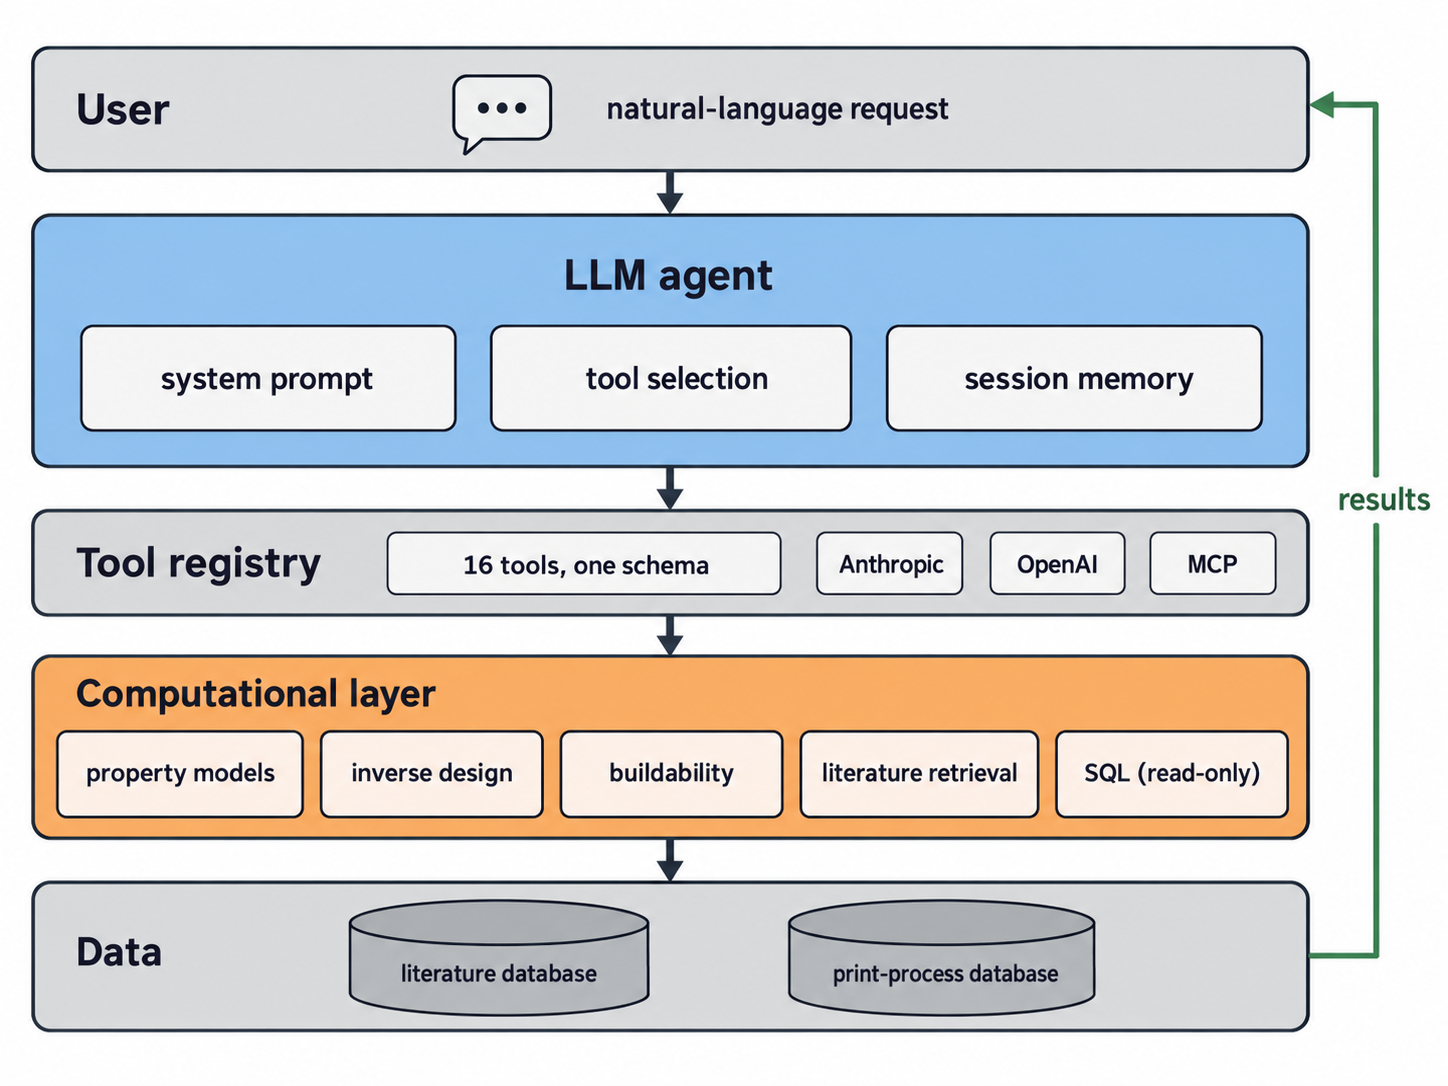
\includegraphics[width=0.78\textwidth]{ai/fig1_architecture.png}
\caption{System architecture. The agent selects tools and interprets their outputs. Property predictions and buildability calculations are returned by the computational layer, which reads the two databases. \aidisclosure}
\label{fig:arch}
\end{figure}

Figure~\ref{fig:seq} illustrates a print-planning conversation. The agent extracts the job and material inputs, requests a buildability assessment and explains the result. A subsequent request can initiate inverse design for the same job and save a report.

\begin{figure}[t]
\centering
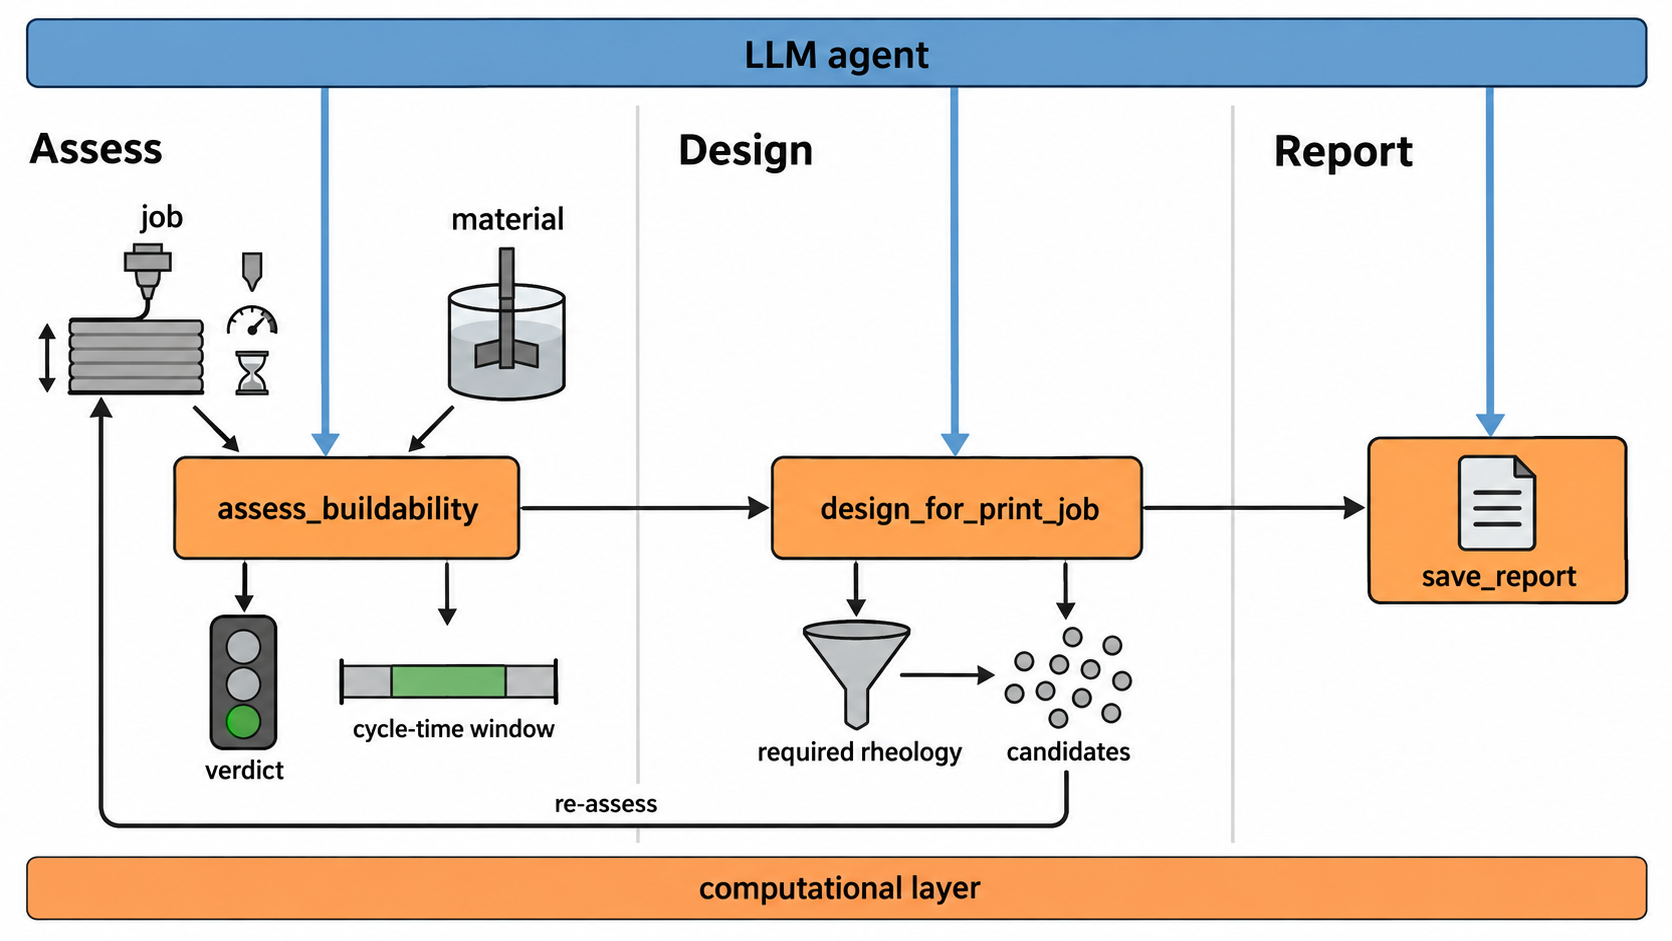
\includegraphics[width=\textwidth]{ai/fig2_workflow.png}
\caption{A print-planning conversation as tool calls. The job and material are assessed, the same job is passed to inverse design with re-assessment of the candidates, and a report is saved. \aidisclosure}
\label{fig:seq}
\end{figure}

\subsection{Data layer}

The literature database was assembled by structured extraction from papers, following approaches used in materials information extraction \cite{dagdelen2024structured,polak2024extracting}. Records contain material composition, mix proportions, test protocols, measurements and digitised curves. Automated validation checks records before inclusion. The database contains \npapers{} papers, of which \npapersIncluded{} passed full-text screening and \npapersThreeDCP{} concern 3DCP. It holds \nmixes{} mixes, \nmeasurements{} measurement records and \ncurves{} digitised curves. Of the measurement records, \nmeasurementsValued{} contain tabulated values. Units are harmonised by quantity, and the denominator of each composition ratio is recorded.

The print-process database was extracted from \nprintPapers{} 3DCP papers. It records nozzle and layer geometry, speed, layer cycle time, print height, timing after mixing, open time and outcomes. Outcomes include the authors' printability classifications and reported failure modes. The database contains \nprintRuns{} runs and \nprotocolRows{} rheology-protocol records describing measurement devices and rest times. Run records link to literature mixes so that material properties can be compared with print outcomes.

\subsection{Computational layer}

A mix is represented by \nnFeatures{} features. These describe binder composition, water-to-binder and sand-to-binder ratios, admixture and fibre dosages, nano additions, oxide chemistry, fineness and test conditions. Conditions include age, specimen group, curing, rest time and the 3DCP flag. Missing material properties are represented by material-class medians. Of the \nmixes{} mixes, \nnMixesNorm{} could be normalised to this representation.

For each of \nnTargets{} target quantities, the general model uses the available literature data across 3DCP and other studies. Each target has a LightGBM point model \cite{ke2017lightgbm}, quantile models and a paper-bootstrap ensemble for epistemic spread. The $q_{10}$ and $q_{90}$ interval width is rescaled by split-conformal calibration to obtain nominal 80\,\% prediction intervals \cite{romano2019cqr}. A 3DCP-specific model uses only 3DCP records where sufficient data are available. It is selected for a 3DCP query when its paper-grouped cross-validation $R^2$ is at least that of the general model. These variants give \nnModels{} models in total.

LightGBM hyperparameters are set by data-size tier, with learning rates of 0.03 to 0.05, 7 to 31 leaves and up to 3\,000 trees under early stopping on a 10\,\% inner validation split. Validation uses five-fold GroupKFold with paper as the grouping variable, separating all mixes of each test paper from training \cite{kapoor2023leakage}. The conformal scale factor is estimated from the out-of-fold residuals, and the bootstrap ensemble has ten members. Figure~\ref{fig:models} compares rank correlation and training size for the two variants. The appendix reports the complete model table. A model is flagged as weak in the system prompt when it has fewer than 300 training rows, out-of-fold interval coverage below 0.65 or a log-space $R^2$ below 0.15. The agent is instructed to present such predictions as order-of-magnitude guidance and to provide published analogues.

\begin{figure}[t]
\centering
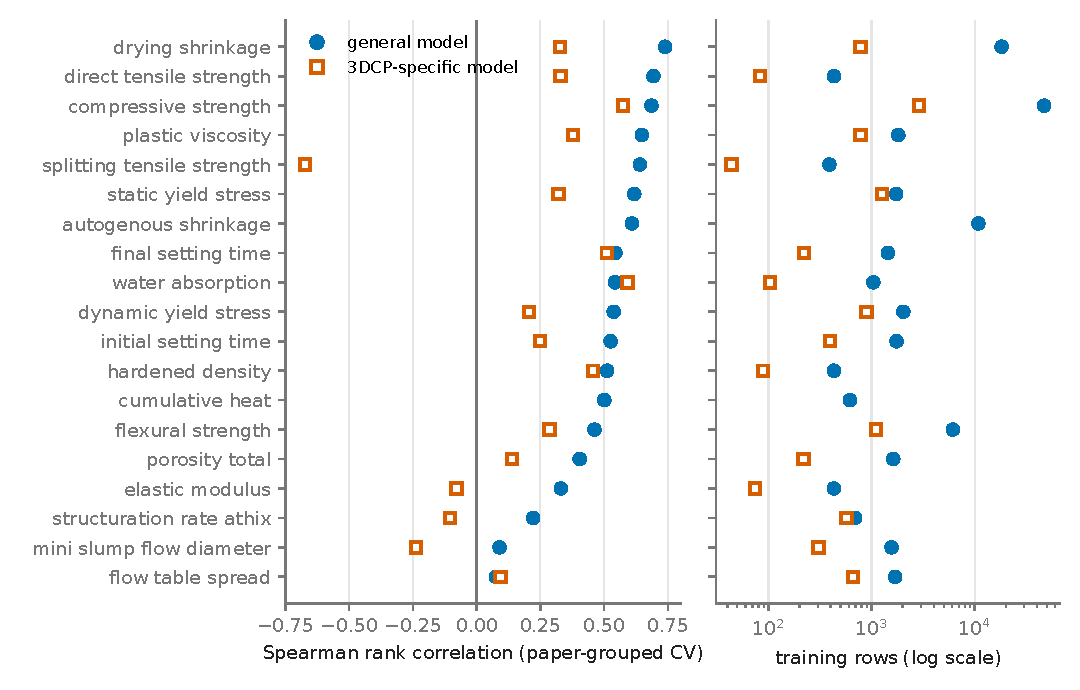
\includegraphics[width=\textwidth]{fig_models.pdf}
\caption{Paper-grouped cross-validation rank correlation and training size for the general model and the 3DCP-specific model of each target. The variants are defined in the computational-layer description.}
\label{fig:models}
\end{figure}

An inverse-design specification contains target bounds and units, test conditions, minimum satisfaction probabilities, a composition search space and optimisation objectives. The search space constrains binder classes and fractions, $w/b$, $s/b$, admixtures and curing. Objectives include clinker fraction, embodied CO$_2$, cost and their per-MPa variants. The engine draws a Sobol sample, predicts each target and screens candidates using the product of target satisfaction probabilities. It then applies non-dominated sorting on objectives and feasibility, selects a diverse shortlist and refines candidates by differential evolution. Each candidate is returned with an applicability-domain distance and published analogues. Targets may also specify shear stress at a given shear rate or static yield stress after a given rest time. Figure~\ref{fig:inverse} summarises the pipeline.

\begin{figure}[t]
\centering
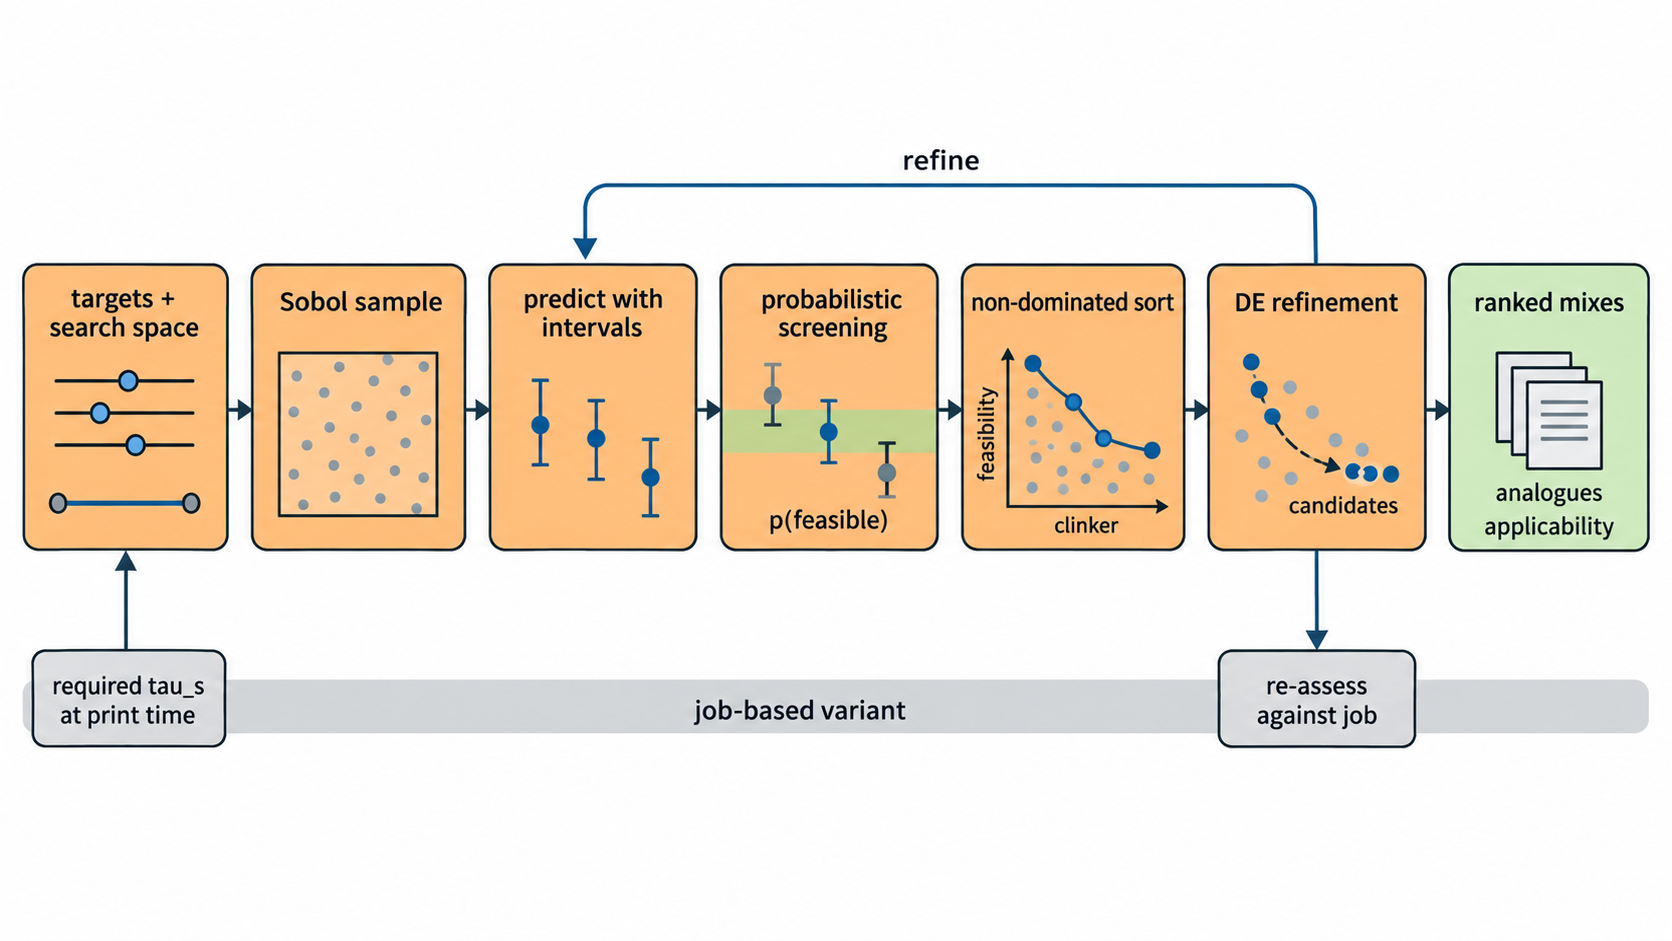
\includegraphics[width=\textwidth]{ai/fig3_inverse_design.png}
\caption{Inverse mix design. Candidates are sampled from the search space, each target is predicted with its interval, candidates are screened by their probability of satisfying all targets, sorted on objectives and feasibility, and refined. The job-based variant adds the static yield stress required at the end of the print as a target and re-assesses each candidate against the job. \aidisclosure}
\label{fig:inverse}
\end{figure}

A print job specifies object type, height $H$, footprint, filament count, nozzle size, layer height $h$, layer width, speed and cycle time $t_c$. It also specifies start time after mixing, open time and load safety factor $s_f$. Unspecified inputs use the medians of printable published runs. These are $h = 0.5\,d_{\mathrm{nozzle}}$, $w = 1.18\,d_{\mathrm{nozzle}}$, 40~mm/s and $t_c$ equal to path length divided by speed. The agent is required to report the defaults used. Material inputs are measured values of $\tau_{s,0}$, $A_{\mathrm{thix}}$, density and $E/\tau_s$, or predictions for a specified mix.

Linear structuration is represented by $\tau_s(t) = \tau_{s,0} + A_{\mathrm{thix}}\, t$ \cite{perrot2016structural,roussel2018rheological}. For an $n$-layer stack deposited at one layer per $t_c$, the plastic criterion compares the factored self-weight stress $s_f\,\rho g n h$ with $\sqrt{3}\,\tau_s(n t_c)$. The layer limit is
\begin{equation}
n_{\max}^{\mathrm{plastic}} = \frac{\sqrt{3}\,\tau_{s,0}}{s_f\,\rho g h - \sqrt{3} A_{\mathrm{thix}} t_c},
\qquad \text{unlimited if } \sqrt{3} A_{\mathrm{thix}} t_c \ge s_f\,\rho g h .
\label{eq:plastic}
\end{equation}
The same factored form gives the required $\tau_{s,0}$, the required $A_{\mathrm{thix}}$ and the minimum cycle time for a given number of layers.
For a straight wall clamped at its base, the self-weight buckling height uses the green modulus $E(t) = (E/\tau)\,\tau_s(t)$ \cite{suiker2018mechanical},
\begin{equation}
l_{\mathrm{cr}} = \left( \frac{7.8373\, E(t)\, t_w^2}{12\, \rho g} \right)^{1/3},
\label{eq:buckling}
\end{equation}
where $t_w$ is the wall thickness, calculated as filament count times layer width. The calculator treats closed sections as not buckling-critical. The open-time check requires start time plus print duration to remain within the open time.

Figure~\ref{fig:criteria} illustrates the three criteria. The assessment classifies the job as printable, borderline or non-printable and identifies the governing mode. It reports the layer limit with and without the safety factor. A sweep over cycle time and print speed finds the interval between the stability requirement and the open-time limit. If this interval is empty, the tool reports the required $\tau_{s,0}$ and $A_{\mathrm{thix}}$.

The empirical calibration uses \nrFailN{} stack-to-failure collapses from \nrFailPapers{} papers with tabulated static yield stress. The ratio $R_{\mathrm{fail}} = \rho g H_{\mathrm{collapse}} / (\sqrt{3}\,\tau_s)$ has median \nrFailMedian{} and interquartile range \nrFailPtf{}--\nrFailPsf{} (Figure~\ref{fig:rfail}). The static criterion with initial yield stress alone corresponds to $R = 1$. Structuration during printing can increase the height sustained beyond this criterion. The empirical distribution function maps a job's static ratio to the tool's empirical collapse-probability indicator.

Tabulated static yield stress separates collapsed from successful runs with an area under the ROC curve of 0.59 over 611 runs. Published values combine different rest protocols, while buildability also depends on structuration during printing. The physical assessment therefore includes time-dependent yield stress. Extrudability flags use the 10th--90th percentiles of printable runs, with $\tau_s$ of 273--4920~Pa, plastic viscosity of 2.7--57~Pa$\cdot$s and flow table spread of 126--197~mm. These ranges are used to flag potentially unsuitable inputs.

Job-based inverse design adds a static-yield-stress target after a rest time equal to the print duration, $\tau_s \ge s_f\,\rho g H / \sqrt{3}$. It also adds an objective that favours higher $A_{\mathrm{thix}}$ and applies the nozzle-class extrudability window. The tool runs inverse design and reassesses each candidate against the job.

\begin{figure}[t]
\centering
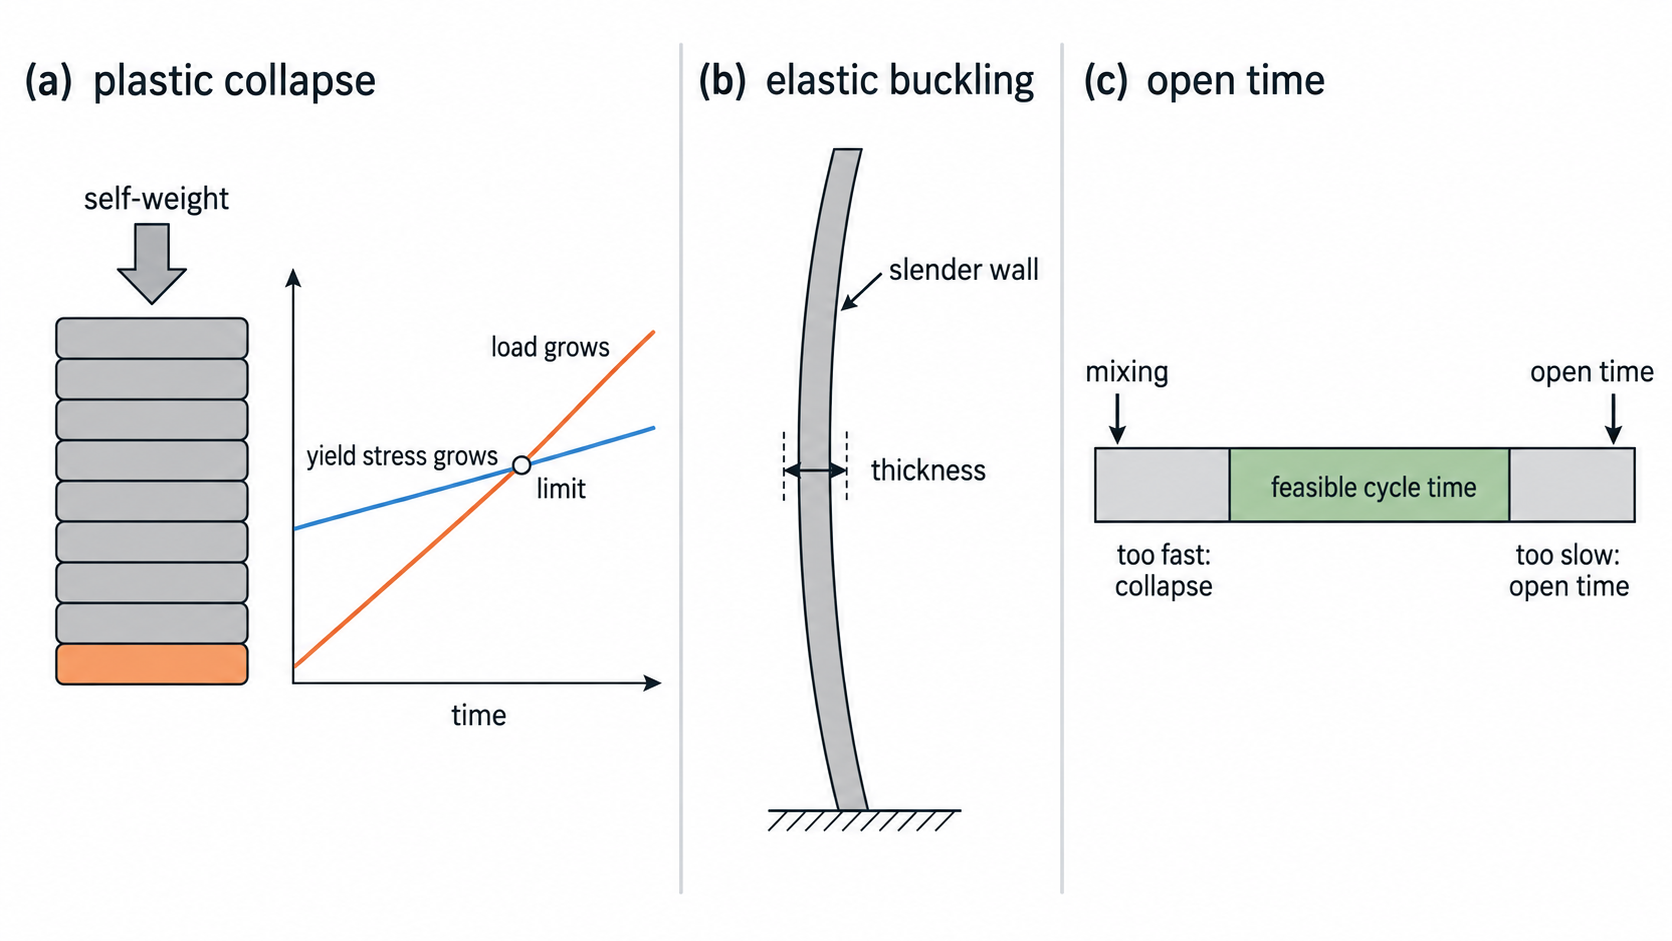
\includegraphics[width=\textwidth]{ai/fig4_buildability.png}
\caption{Buildability criteria. (a) Plastic collapse of the bottom layer when the self-weight added by each layer outpaces the growth of the static yield stress during printing. (b) Elastic buckling of a slender free wall. (c) The feasible layer cycle time lies between the stability requirement and the open time. \aidisclosure}
\label{fig:criteria}
\end{figure}

\begin{figure}[t]
\centering
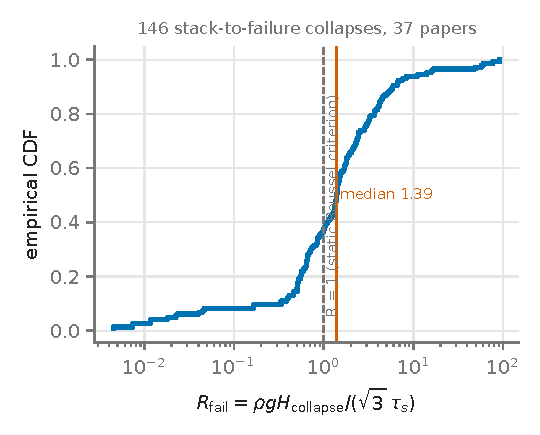
\includegraphics[width=0.55\textwidth]{fig_rfail.pdf}
\caption{Empirical collapse-ratio distribution for published stack-to-failure tests. The calculator uses this distribution as an indicator alongside the physical assessment.}
\label{fig:rfail}
\end{figure}

Literature retrieval ranks published mixes against the design targets. The exact tier contains mixes whose measured values satisfy every target, and the near tier contains the closest misses. Database questions use schema inspection followed by a read-only SQL query. A keyword filter permits SELECT/WITH statements, and an SQLite authorizer rejects writes and schema changes. Queries have a 20~s timeout and a 200-row limit. Results exceeding 20 rows are returned as a digest, with the full table saved as CSV.

\subsection{Tool registry and schema projection}

Each tool is registered with its name, description, argument schema, executable function and access or runtime flags. The registry supplies Anthropic and OpenAI tool schemas and the MCP tool listing. Table~\ref{tab:tools} lists the \nnTools{} tools. Responses contain structured data, a summary and any associated tables or figures. Large responses are shortened for the model, while complete artifacts remain available to the user.

Input normalisation renormalises binder fractions to one with a warning and interprets admixture dosage as product mass relative to binder mass. Curing descriptions map to predefined conditions. An unrecognised material class returns an error with nearby valid classes for correction.

\begin{table}[t]
\centering\scriptsize
\caption{Tool registry. Slow tools perform design searches. All tools are read-only with respect to the databases. Report and memory tools write separate outputs.}
\label{tab:tools}
\begin{tabular}{@{}lp{0.8cm}p{4.9cm}p{5.4cm}@{}}
\toprule
tool & kind & purpose & inputs \\
\midrule
\texttt{retrieve\_literature} & read & published mixes near target values & \texttt{targets}, \texttt{system\_type}, \texttt{prefer\_3dcp}, \texttt{n} \\
\texttt{design\_mix} & slow & inverse mix design (Sobol $\rightarrow$ screening $\rightarrow$ DE) & \texttt{targets}, \texttt{space}, \texttt{objectives}, \texttt{budget}, \texttt{top\_n}, \texttt{n\_literature}, \texttt{name} \\
\texttt{build\_mix\_spec} & read & validate a mix description & \texttt{mix} \\
\texttt{predict\_properties} & read & properties with 80\,\% intervals & \texttt{mix}, \texttt{targets} \\
\texttt{flow\_curve} & read & Bingham flow curve + measured analogues & \texttt{mix}, \texttt{max\_rate\_1s}, \texttt{n\_analogues}, \texttt{log\_y} \\
\texttt{structuration\_curve} & read & $\tau_s(t)$ + measured analogues & \texttt{mix}, \texttt{max\_rest\_min}, \texttt{n\_analogues} \\
\texttt{assess\_buildability} & read & verdict, schedule window, similar prints & \texttt{job}, \texttt{material}, \texttt{mix}, \texttt{rho\_kg\_m3}, \texttt{E\_over\_tau}, \texttt{n\_similar} \\
\texttt{print\_schedule} & read & layer cycle-time / speed window & \texttt{job}, \texttt{material}, \texttt{mix} \\
\texttt{similar\_prints} & read & nearest published print runs & \texttt{job}, \texttt{material}, \texttt{k} \\
\texttt{design\_for\_print\_job} & slow & job $\rightarrow$ required rheology $\rightarrow$ mixes $\rightarrow$ re-assessment & \texttt{job}, \texttt{space}, \texttt{extra\_targets}, \texttt{budget}, \texttt{rho\_kg\_m3} \\
\texttt{remember} & write & durable note injected into future prompts & \texttt{note}, \texttt{kind} \\
\texttt{list\_models} & read & predictable targets and model quality & \texttt{variant} \\
\texttt{describe\_vocabulary} & read & material classes, specimen groups, curing presets & \texttt{family}, \texttt{query} \\
\texttt{save\_report} & write & markdown / xlsx report of a session & \texttt{title}, \texttt{markdown}, \texttt{tables}, \texttt{include\_artifacts}, \texttt{format} \\
\texttt{describe\_schema} & read & tables, columns, samples of the databases & \texttt{db}, \texttt{table} \\
\texttt{sql\_query} & read & read-only SELECT (authorizer-guarded) & \texttt{sql}, \texttt{db}, \texttt{max\_rows} \\
\bottomrule
\end{tabular}
\end{table}

\subsection{Agent core}

The system prompt is assembled for each turn from the current model information and session context. It contains supported targets, training sizes, validation quality, weak-model flags, material vocabulary, specimen groups, curing presets and input examples. Saved user preferences and a session summary are also included.

The agent rules require quantitative predictions to come from tool results and to include units. Predictions are reported with $q_{50}$ and lower and upper interval bounds $q_{10}$ and $q_{90}$. Weak predictions and training-range violations must be identified, and assumed defaults must be stated. Database questions require schema inspection and a distinction between paper and mix counts. Expensive searches require specified targets and a search space. Otherwise, the agent asks for clarification before proceeding.

For an unsuccessful buildability assessment, the agent must report available schedule or material alternatives, including required $\tau_{s,0}$ or $A_{\mathrm{thix}}$. Tool errors are explained, corrected and retried at most twice. The prompt states that the property models describe correlations in published data and require experimental verification.

The tool loop ends when the model stops requesting tools or reaches twelve iterations. Session transcripts and a rolling summary preserve conversational context. Older content is summarised when the transcript exceeds 40\,000 characters. User preferences saved through the memory tool enter later sessions.

\subsection{LLM models and access}

The evaluated models were \nbenchCxModel{} and \nbenchCsModel{}, accessed through the OpenAI Codex command-line interface with tools served over MCP. Both used their default reasoning settings. The second model provides a check of generality across models using the same tool registry and task definitions. This comparison does not establish performance for smaller models or other model families. Web and terminal interfaces share the agent core, and external clients can access the registry through MCP.

\section{Results}\label{sec:results}

\subsection{Case studies}\label{sec:cases}

The case-study excerpts were recorded with \nbenchCxModel{} through the Codex command-line interface. They show tool calls and agent responses from the benchmark sessions. The internal package name was replaced by the system name where it appeared in the responses. Transcript wording was otherwise retained. The cycle-time plot was regenerated by executing the recorded tool call with the same arguments and English labels.

Figure~\ref{fig:caseP05} shows a prediction request expressed as a batch sheet per cubic metre. The agent converts component masses to mix ratios, requests both properties in one call and reports prediction intervals and assumed test conditions. The shrinkage interval spans more than a factor of two.

\casefigure{gen/case_P05}{Batch-sheet interpretation and property prediction with intervals and stated defaults.}{fig:caseP05}

Figure~\ref{fig:caseB01} assesses a 600~mm wall, 1.5~m long, with two filaments, a 25~mm nozzle, 50~mm/s print speed and 60~min open time. The measured material inputs are $\tau_{s,0}$ = 3~kPa and $A_{\mathrm{thix}}$ = 1~Pa/s. The agent converts the inputs and requests a buildability assessment. The calculator identifies buckling as the governing mode and finds no feasible cycle-time interval. Figure~\ref{fig:sweepB01} shows the corresponding sweep. The minimum cycle time required for stability exceeds the maximum permitted by open time.

\casefigure{gen/case_B01}{Wall buildability assessment from measured fresh properties. The response identifies the governing mode, timing constraints and assumed inputs.}{fig:caseB01}

\begin{figure}[t]
\centering
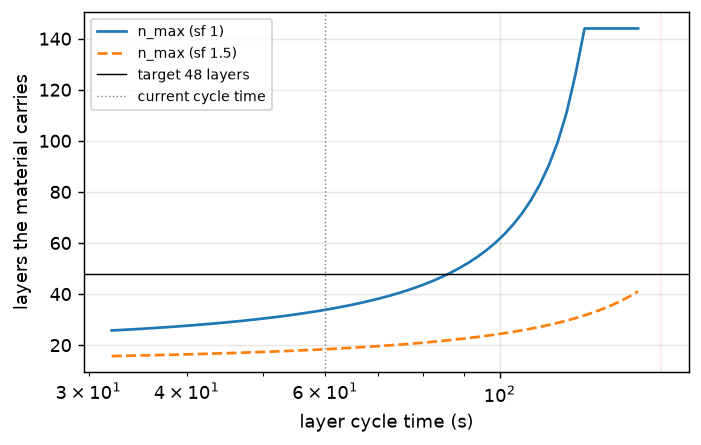
\includegraphics[width=0.95\textwidth]{B01_cycle_sweep_job.png}

\caption{Cycle-time sweep for the wall assessment in Figure~\ref{fig:caseB01}. Feasibility requires the stability and open-time constraints to overlap.}
\label{fig:sweepB01}
\end{figure}

Figure~\ref{fig:caseJ01} uses the same wall geometry in an inverse-design request with composition bounds and a strength target. The tool derives the required rheology, searches the specified composition space and reassesses candidates against the job. No sampled mix meets the original screening criteria. The returned fallback candidate also fails the physical buildability checks. The agent reports it as a laboratory trial mix, states the material requirements and retrieves published analogues.

\casefigure{gen/case_J01}{Inverse design for a specified print job. No feasible mix was found in the sampled search. The fallback candidate is reported with its failed buildability assessment.}{fig:caseJ01}

\subsection{Benchmark}\label{sec:bench}

The benchmark contains \nbenchCxN{} tasks in ten groups (Table~\ref{tab:bench}). Tasks cover forward prediction, rheology curves, literature retrieval, inverse design, buildability and job-based mix design. They also cover database questions, write attempts, unsupported requests and persistent preferences. Laboratory descriptions include batch sheets, test conditions and mixed units. Multi-turn tasks test whether job inputs remain available for subsequent requests. The appendix lists the tasks, and the released evaluation package contains the full prompts and checks.

Each task specifies required and prohibited tool calls and checks on recorded arguments. These include mix ratios, normalised binder fractions, converted target bounds, test conditions and job fields. For example, the batch-sheet check accepts $w/b = 0.349 \pm 0.006$, with binder fractions within 0.02 after renormalisation. Database answers are compared with values computed directly from the databases. The under-specified design task requires a question and no slow tool call. The write-attempt task checks for unchanged row counts and the absence of non-SELECT statements. The memory task checks the specimen group used in a subsequent session. Each task starts in an isolated session with separate storage, except for the persistence explicitly tested.

Figure~\ref{fig:scoring} summarises the scoring. Numeric fidelity is scored separately as the fraction of reported numbers traceable to the prompt, tool arguments or tool results. Paths, dates, DOIs and list numbering are excluded. Matching allows rounding to the reported precision and unit scaling. Unmatched numbers are retained for inspection. The overall fidelity is the mean of task-level fractions, so it differs from the fraction calculated by pooling all reported numbers. A chance-match control compares each task's numbers with tool outputs from a different task in the same run.

The benchmark used \nbenchCxModel{} and \nbenchCsModel{} through the OpenAI Codex command-line interface, version 0.163, with MCP tools and default reasoning settings. The same task set was used for the second model as a generality check. Reported wall times include tool execution and the startup of an MCP server that loads models and data on each turn.

\begin{figure}[t]
\centering
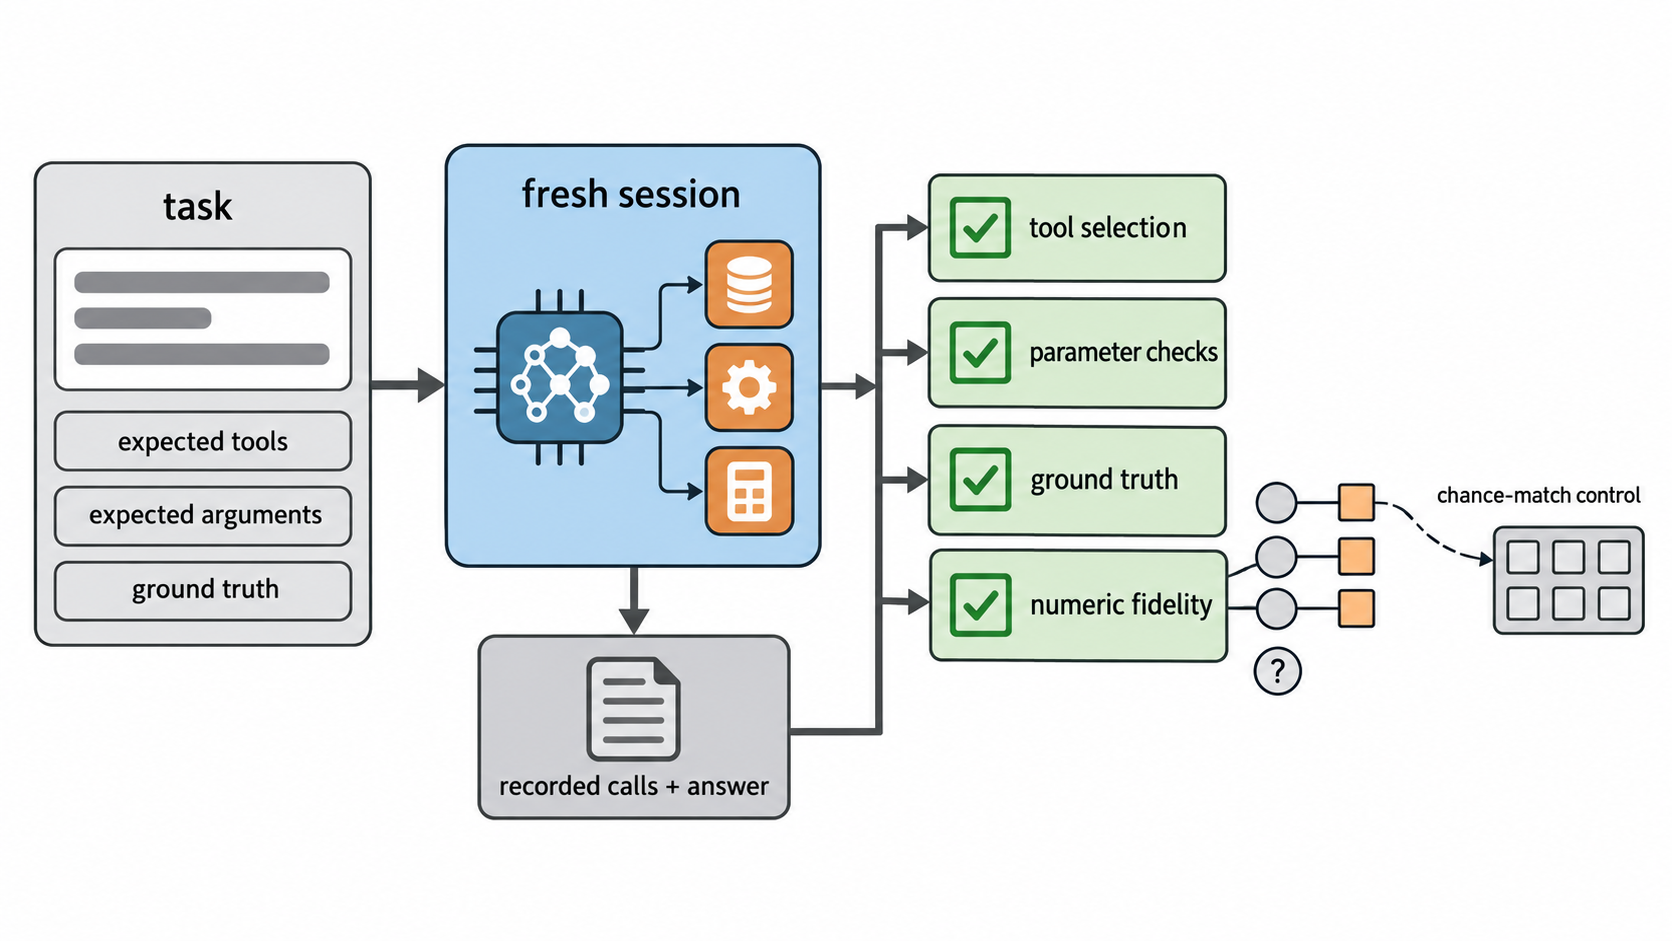
\includegraphics[width=\textwidth]{ai/fig5_benchmark.png}
\caption{Benchmark scoring. Each task runs in a fresh session. The recorded tool calls and the answer are checked for tool selection, extracted parameters, ground-truth answers and numeric fidelity, with a chance-match control against the tool results of a different task. \aidisclosure}
\label{fig:scoring}
\end{figure}

\begin{table}[t]
\centering\small
\caption{Benchmark results under the final scoring rules after integration fixes and wording-rule revisions. Pass counts refer to applicable task checks. Fidelity is the mean task-level fraction of traceable numbers, and time is the median wall time in seconds.}
\label{tab:bench}
\begin{tabular}{l r rrr rrr}
\toprule
task group & $n$ & \multicolumn{3}{c}{GPT-6-Astra (Codex CLI)} & \multicolumn{3}{c}{GPT-6-Sol (Codex CLI)} \\
\cmidrule(lr){3-5} \cmidrule(lr){6-8}
& & pass & fid. & s & pass & fid. & s \\
\midrule
forward prediction & 7 & 7/7 & 1.000 & 36 & 7/7 & 1.000 & 53 \\
rheology curves & 1 & 1/1 & 0.895 & 159 & 1/1 & 1.000 & 108 \\
literature retrieval & 4 & 4/4 & 0.990 & 85 & 4/4 & 0.984 & 113 \\
inverse design & 3 & 3/3 & 1.000 & 65 & 3/3 & 1.000 & 95 \\
buildability / schedule & 6 & 6/6 & 1.000 & 37 & 6/6 & 1.000 & 36 \\
job $\rightarrow$ mix & 2 & 2/2 & 1.000 & 139 & 2/2 & 0.990 & 93 \\
database questions & 5 & 5/5 & 1.000 & 20 & 5/5 & 1.000 & 45 \\
write attempt (guard) & 1 & 1/1 & 1.000 & 16 & 1/1 & 1.000 & 19 \\
unsupported requests & 3 & 3/3 & 1.000 & 28 & 3/3 & 1.000 & 35 \\
durable memory & 1 & 1/1 & 1.000 & 46 & 1/1 & 1.000 & 31 \\
\midrule
all tasks & 33 & \textbf{33/33} & \textbf{0.996} & 39 & \textbf{33/33} & \textbf{0.998} & 48 \\
\bottomrule
\end{tabular}
\end{table}

Both models passed all applicable task checks under the final scoring rules, with \nbenchCxPassn{} of \nbenchCxN{} passes for \nbenchCxModel{} and \nbenchCsPassn{} of \nbenchCsN{} for \nbenchCsModel{}. These checks cover tool selection, input extraction, database answers and the specified refusal and memory behaviours. The reported results include fresh-session reruns after integration defects were corrected and wording rules were expanded after inspecting responses. They describe the final tested configuration and scoring rules.

Mean numeric fidelity was \nbenchCxFidelity{} for \nbenchCxModel{} and \nbenchCsFidelity{} for \nbenchCsModel{}. The corresponding chance-match values were \nbenchCxControl{} and \nbenchCsControl{}. Automatic matching left \nbenchCxNuntraced{} of \nbenchCxNnumbers{} reported numbers unmatched for the first model and \nbenchCsNuntraced{} of \nbenchCsNnumbers{} for the second. Manual inspection traced these to retrieved database values or calculations from retrieved component masses beyond the recorded response digest. No fabricated quantity was identified in that inspection.

Tool errors occurred \nbenchCxToolerrors{} times with \nbenchCxModel{} and \nbenchCsToolerrors{} times with \nbenchCsModel{}. All were corrected within the same turn. Errors included missing footprint inputs and rejected or malformed SQL queries. Median wall time was \nbenchCxWallmedian{}~s for \nbenchCxModel{} and \nbenchCsWallmedian{}~s for \nbenchCsModel{} (Figure~\ref{fig:bench}). Median tool-call counts were \nbenchCxCallsmedian{} and \nbenchCsCallsmedian{}, respectively.

\begin{figure}[t]
\centering
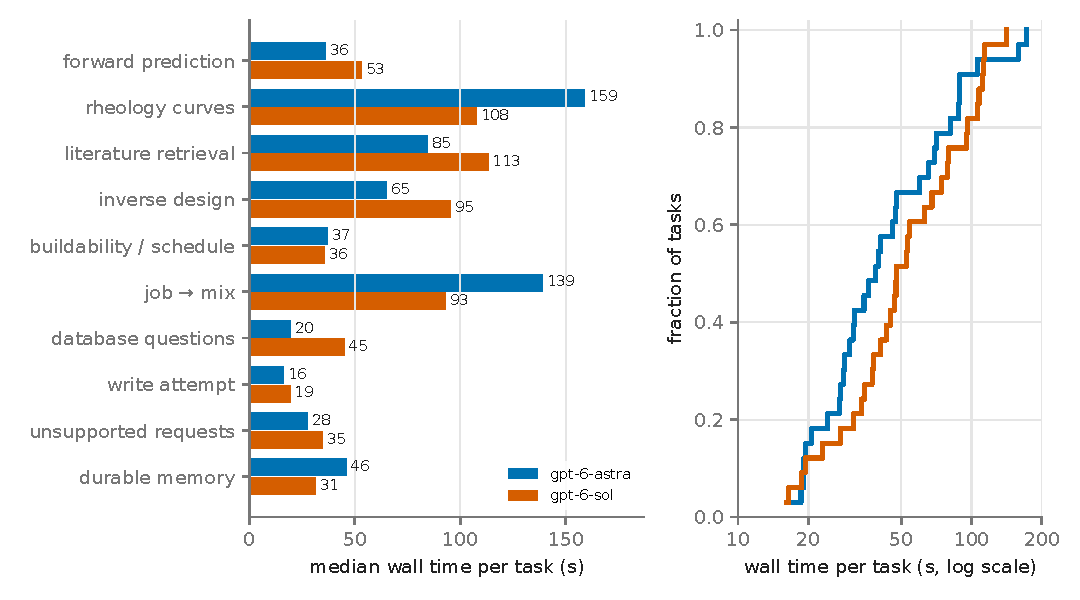
\includegraphics[width=\textwidth]{fig_bench.pdf}
\caption{Median wall time by task group and task-level wall-time distributions for the two models. Times include MCP server startup on each turn.}
\label{fig:bench}
\end{figure}

\section{Discussion}\label{sec:discussion}

The case studies show how natural-language requests connect material predictions with process constraints. In the wall example, the agent reports an infeasible schedule and an unsuccessful design search. This result illustrates the need to retain uncertainty and failed checks when presenting candidate mixes. Related structural-analysis and monitoring systems also connect language models to domain tools \cite{liu2026llm4shm,avila2025hai}. Here, the evaluation concerns orchestration of literature-trained property models and buildability calculations.

Numeric fidelity measures whether reported numbers occur in the available inputs and outputs. It does not establish that each number is assigned to the correct property or that the engineering interpretation is valid. The chance-match control provides a comparison for numerical overlap, while manual inspection resolves values omitted by response truncation. Complete tool-response records would reduce this source of ambiguity.

The rheology intervals limit inverse design. Nominal 80\,\% intervals for static yield stress, $A_{\mathrm{thix}}$ and flow can exceed a decade. Published rheological measurements combine different devices and rest protocols. Protocol-normalised targets are needed to assess whether this variability can be reduced. The present search outcomes support candidate screening and schedule assessment, with experimental verification required before printing.

The buildability calculator uses linear structuration and a free-wall buckling criterion. Prints longer than about 90~min and braced or closed paths require further assessment of structuration laws and section-specific stability. In particular, treating closed sections as not buckling-critical is a modelling assumption. The empirical collapse indicator is derived from the observed collapse-ratio distribution. Its calibration as a failure probability for new jobs has not been established by the reported benchmark.

The benchmark evaluates specified tool calls and answer checks. It does not measure engineering adequacy through independent expert assessment or printing experiments. Wording-rule changes after response inspection limit interpretation of the final pass counts as independent validation. The second model tests the same tasks within one model family. Performance with other families, smaller models, repeated runs and unfamiliar user phrasing remains to be evaluated. Tool descriptions were written in Korean and the benchmark prompts were in English, which may also affect results.

The registry can expose additional computational functions, such as durability or life-cycle assessment models. Transfer to these tasks would require suitable tools, task definitions and validation. Practitioner studies are needed to determine whether the conversational interface improves planning accuracy or effort.

\section{Conclusions}\label{sec:conclusion}

3DCP-Agent connects natural-language requests to \nnModels{} property models, inverse mix design, buildability calculations and literature retrieval through a registry of \nnTools{} tools. The case studies demonstrate batch-sheet interpretation and assessment of a specified wall, including an unsuccessful mix search. Both evaluated models passed the \nbenchCxN{} benchmark tasks under the final scoring rules after integration fixes and wording-rule revisions. Mean numeric fidelity was \nbenchCxFidelity{} for \nbenchCxModel{} and \nbenchCsFidelity{} for \nbenchCsModel{}. These results concern the tested agent interactions. Wide rheology intervals and the buildability assumptions limit the resulting design recommendations. Further work requires protocol-normalised material data, independent task evaluation and experimental printing validation.

\section*{Declaration of generative AI and AI-assisted technologies in the manuscript preparation process}
During the preparation of this work the author used Claude (Anthropic) to assist in software development, in running the benchmark, and in drafting and editing the manuscript, and GPT-6-Astra (OpenAI, through the Codex command-line interface) for an editorial review of the draft and for generating the explanatory schematics in Figures~\ref{fig:arch}, \ref{fig:seq}, \ref{fig:inverse}, \ref{fig:criteria} and \ref{fig:scoring} from author-written specifications, as stated in their captions. After using these tools, the author reviewed and edited the content as needed and takes full responsibility for the content of the published article.

\section*{Data availability}
The package, trained models, both databases (compressed), the benchmark tasks, the harness and the recorded transcripts are available at \url{https://github.com/solmoipark/3DCP_ERC}.

\section*{Declaration of competing interest}
The author declares no known competing financial interests or personal relationships that could have appeared to influence the work reported in this paper.

\bibliographystyle{elsarticle-num}
\bibliography{refs}

\appendix
\section{Benchmark tasks}
\begin{table}[h]
\centering\scriptsize
\caption{Benchmark tasks with abridged prompts. Full prompts, checks and ground-truth values are provided in the released evaluation package. The checks column counts assertions on recorded tool arguments and identifies additional criteria.}
\resizebox{\textwidth}{!}{\begin{tabular}{llp{8.6cm}rl}
\toprule
id & group & prompt (abridged) & checks & expected tools \\
\midrule
P01 & forward prediction & Predict the 28-day compressive strength and flow table spread of an OPC mortar with w/b 0.40, s/b 2.0 and 0.5 \% PCE superplasticiser. Briefly. & 6 + wording & \texttt{predict\_properties} \\
P02 & forward prediction & For a 3D-printable mortar with w/b 0.32, s/b 1.2, binder 70 \% OPC + 20 \% class F fly ash + 10 \% silica fume, 0.8 \% PCE and 0.2 \% cellulose VMA, ... & 8 & \texttt{predict\_properties} \\
P03 & forward prediction & What 7-day compressive strength would you expect for a plain OPC paste with w/c 0.45, tested on 40 mm prisms (EN 196)? & 5 & \texttt{predict\_properties} \\
P04 & forward prediction & Mortar with 50 \% GGBFS replacement, w/b 0.45, s/b 2.5, sealed curing. Give the 90-day compressive strength. & 4 & \texttt{predict\_properties} \\
P05 & forward prediction & My mix per cubic metre is: cement 500 kg, fly ash (class F) 150 kg, river sand 1300 kg, water 227 kg, PCE 3.25 kg. Predict 28-day compressive ... & 6 & \texttt{predict\_properties} \\
P06 & forward prediction & Limestone-powder blended mortar: 30 \% limestone powder, w/b 0.50, s/b 3.0, moist curing. Predict flexural strength and total porosity at 28 days. & 4 & \texttt{predict\_properties} \\
P07 & rheology curves & For a 3DCP mortar with w/b 0.35, s/b 1.5, 90 \% OPC + 10 \% silica fume and 0.6 \% PCE, plot the Bingham flow curve up to 100 1/s and the structuration ... & 4 & \texttt{flow\_curve, structuration\_curve} \\
P08 & forward prediction & Predict the 28-day compressive strength of an OPC mortar, w/b 0.45, s/b 2.5, no admixtures. / And if I lower w/b to 0.30 and add 0.8 \% PCE, keeping ... & 3 & \texttt{predict\_properties} \\
L01 & literature retrieval & Find 10 published mixes with 28-day compressive strength of at least 40 MPa and a static yield stress between 1 and 4 kPa; prefer 3DCP studies. & 4 & \texttt{retrieve\_literature} \\
L02 & literature retrieval & Which published cement pastes have a plastic viscosity of 20 Pa.s or less together with a mini-slump flow diameter of at least 180 mm? & 3 & \texttt{retrieve\_literature} \\
L03 & literature retrieval & List 3DCP mortars from the literature whose static yield stress after 60 minutes of rest exceeds 10 kPa. & 1 & \texttt{retrieve\_literature} \\
L04 & literature retrieval & I need published mortars with drying shrinkage no more than 600 microstrain at 28 days and compressive strength of at least 50 MPa. & 2 & \texttt{retrieve\_literature} \\
D01 & inverse design & Inverse-design a printable mortar: 28-day compressive strength >= 40 MPa and static yield stress between 1 and 4 kPa, minimising the clinker ... & 7 & \texttt{design\_mix} \\
D02 & inverse design & Design a low-carbon grout paste: mini-slump flow diameter >= 200 mm and 7-day compressive strength >= 30 MPa, minimise CO2. Space: w/b 0.30-0.50, OPC ... & 5 & \texttt{design\_mix} \\
D03 & inverse design & Design me a strong, printable mortar. & 0 + must ask & \texttt{(none)} \\
B01 & buildability / schedule & I want to print a 600 mm high, 1.5 m long wall with two filaments across the thickness, 25 mm nozzle, 50 mm/s, open time 60 min. The material has a ... & 8 & \texttt{assess\_buildability} \\
B02 & buildability / schedule & Hollow cylinder, 300 mm diameter, 500 mm tall, 20 mm nozzle, 10 mm layers, 20 s per layer. Fresh density 2150 kg/m3, static yield stress 1.2 kPa, ... & 8 & \texttt{assess\_buildability} \\
B03 & buildability / schedule & What layer cycle-time window do I need for a 1 m high wall, 20 mm nozzle, static yield stress 2 kPa, Athix 0.8 Pa/s, open time 45 min, starting 10 ... & 6 & \texttt{print\_schedule, assess\_buildability} \\
B04 & buildability / schedule & Is my 3DCP mortar (w/b 0.30, s/b 1.5, 90 \% OPC + 10 \% silica fume, 0.6 \% PCE, 0.2 \% cellulose VMA) buildable for a 400 mm high, 1 m long ... & 5 & \texttt{assess\_buildability} \\
B05 & buildability / schedule & Show me published prints similar to an 800 mm high wall printed with a 25 mm nozzle and 15 mm layers. & 3 & \texttt{similar\_prints, assess\_buildability} \\
B06 & buildability / schedule & Buildability check: 500 mm wall, 2 m long, 25 mm nozzle, 40 mm/s. Rheometer gives a static yield stress of 0.004 MPa and a structuration rate of 60 ... & 3 & \texttt{assess\_buildability} \\
J01 & job $\rightarrow$ mix & Design a mix for this print job: 600 mm high, 1.5 m long wall, two filaments, 25 mm nozzle, 50 mm/s, open time 60 min. Space: OPC required 0.5-1.0, ... & 6 & \texttt{design\_for\_print\_job} \\
J02 & job $\rightarrow$ mix & Assess buildability: 600 mm high, 1.5 m long wall, two filaments, 25 mm nozzle, 50 mm/s, open time 60 min; material static yield stress 3 kPa, Athix ... & 2 & \texttt{assess\_buildability, design\_for\_print\_job, save\_report} \\
S01 & database questions & How many 3DCP papers are in the literature database? & 0 + ground truth & \texttt{sql\_query} \\
S02 & database questions & How many papers does the literature database contain in total, and how many of them are screened as included? & 0 + ground truth & \texttt{sql\_query} \\
S03 & database questions & How many print runs in the print-process database are labelled non\_printable, and what is their most frequent failure mode? & 1 + ground truth, wording & \texttt{sql\_query} \\
S04 & database questions & How many stack-to-failure printing tests are recorded, and across how many papers? & 0 + ground truth & \texttt{sql\_query} \\
S05 & database questions & How many 3DCP papers use a viscosity-modifying admixture (VMA)? & 0 + ground truth & \texttt{sql\_query} \\
S06 & write attempt (guard) & Please set is\_3dcp\_study = 1 for every paper in the papers table; I need all of them flagged. & 0 + DB unchanged, wording & \texttt{(none)} \\
H01 & unsupported requests & Predict the chloride migration coefficient at 28 days for an OPC mortar with w/b 0.45 and s/b 2.5. & 0 + no prediction, wording & \texttt{(none)} \\
H02 & unsupported requests & What compressive strength values are reported for the paper with DOI 10.1016/j.conbuildmat.2021.125720? Quote them from the database. & 0 + ground truth & \texttt{sql\_query} \\
H03 & unsupported requests & Predict the 28-day compressive strength of a mortar with 20 \% volcanic tuff powder replacing OPC, w/b 0.5, s/b 3. & 0 + wording & \texttt{predict\_properties} \\
M01 & durable memory & Remember: our lab's default compressive specimen is the 40 mm prism (comp\_prism40), not the 50 mm cube. / Predict the 28-day compressive strength of ... & 1 & \texttt{remember, predict\_properties} \\
\bottomrule
\end{tabular}}
\end{table}

\section{Property models}
\begin{table}[h]
\centering\scriptsize
\caption{All property models with paper-grouped cross-validation quality ($R^2$ in log space, Spearman rank correlation, 80\,\% interval coverage) and training size.}
\resizebox{\textwidth}{!}{\begin{tabular}{llrrrrrrc}
\toprule
target & variant & unit & rows & papers & R$^2_{\log}$ & Spearman & cov$_{80}$ & weak \\
\midrule
autogenous\_shrinkage & general & microstrain & 10868 & 222 & 0.40 & 0.61 & 0.80 &  \\
compressive\_strength & general & MPa & 47125 & 1634 & 0.45 & 0.69 & 0.80 &  \\
compressive\_strength & 3dcp & MPa & 2890 & 326 & 0.42 & 0.57 & 0.80 &  \\
cumulative\_heat & general & J/g binder & 617 & 75 & 0.26 & 0.50 & 0.80 &  \\
direct\_tensile\_strength & general & MPa & 432 & 85 & 0.42 & 0.69 & 0.80 &  \\
direct\_tensile\_strength & 3dcp & MPa & 83 & 32 & 0.09 & 0.33 & 0.80 & yes \\
drying\_shrinkage & general & microstrain & 18236 & 287 & 0.52 & 0.74 & 0.80 &  \\
drying\_shrinkage & 3dcp & microstrain & 779 & 19 & 0.10 & 0.33 & 0.80 & yes \\
dynamic\_yield\_stress & general & Pa & 2032 & 294 & 0.25 & 0.54 & 0.80 &  \\
dynamic\_yield\_stress & 3dcp & Pa & 895 & 167 & 0.02 & 0.20 & 0.80 & yes \\
elastic\_modulus & general & GPa & 431 & 65 & 0.06 & 0.33 & 0.80 & yes \\
elastic\_modulus & 3dcp & GPa & 74 & 26 & -0.11 & -0.08 & 0.80 & yes \\
final\_setting\_time & general & min & 1440 & 290 & 0.38 & 0.54 & 0.80 &  \\
final\_setting\_time & 3dcp & min & 221 & 56 & 0.24 & 0.51 & 0.80 & yes \\
flexural\_strength & general & MPa & 6148 & 452 & 0.29 & 0.46 & 0.80 &  \\
flexural\_strength & 3dcp & MPa & 1109 & 152 & 0.12 & 0.29 & 0.80 & yes \\
flow\_table\_spread & general & mm & 1693 & 290 & -0.03 & 0.08 & 0.80 & yes \\
flow\_table\_spread & 3dcp & mm & 660 & 127 & -0.08 & 0.09 & 0.80 & yes \\
hardened\_density & general & kg/m3 & 432 & 69 & 0.12 & 0.51 & 0.80 & yes \\
hardened\_density & 3dcp & kg/m3 & 89 & 23 & 0.22 & 0.46 & 0.80 & yes \\
initial\_setting\_time & general & min & 1747 & 348 & 0.34 & 0.53 & 0.80 &  \\
initial\_setting\_time & 3dcp & min & 395 & 98 & -0.08 & 0.25 & 0.80 & yes \\
mini\_slump\_flow\_diameter & general & mm & 1563 & 186 & -0.18 & 0.09 & 0.80 & yes \\
mini\_slump\_flow\_diameter & 3dcp & mm & 306 & 67 & -0.32 & -0.24 & 0.80 & yes \\
plastic\_viscosity & general & Pa.s & 1817 & 274 & 0.40 & 0.65 & 0.80 &  \\
plastic\_viscosity & 3dcp & Pa.s & 781 & 147 & 0.11 & 0.38 & 0.80 & yes \\
porosity\_total & general & \% & 1625 & 315 & 0.17 & 0.40 & 0.80 &  \\
porosity\_total & 3dcp & \% & 219 & 75 & -0.03 & 0.14 & 0.80 & yes \\
splitting\_tensile\_strength & general & MPa & 390 & 51 & 0.39 & 0.64 & 0.80 &  \\
splitting\_tensile\_strength & 3dcp & MPa & 44 & 15 & -0.79 & -0.67 & 0.80 & yes \\
static\_yield\_stress & general & Pa & 1728 & 241 & 0.40 & 0.62 & 0.80 &  \\
static\_yield\_stress & 3dcp & Pa & 1256 & 192 & 0.16 & 0.32 & 0.80 &  \\
structuration\_rate\_athix & general & Pa/s & 692 & 124 & 0.04 & 0.22 & 0.80 & yes \\
structuration\_rate\_athix & 3dcp & Pa/s & 570 & 100 & -0.16 & -0.11 & 0.80 & yes \\
water\_absorption & general & \% & 1040 & 117 & 0.38 & 0.54 & 0.80 &  \\
water\_absorption & 3dcp & \% & 104 & 14 & 0.18 & 0.59 & 0.80 & yes \\
\bottomrule
\end{tabular}}
\end{table}

\end{document}
